\section{Case Study and Performance Evaluation}
\label{sec:experiments}

\subsection{Dataset and Experimental Setup}
\label{subsec:exp_setup}

We evaluate PhysFormer on a real VPP dataset built from aggregated regional measurements of a distributed energy cluster in Germany. The dataset contains 15-minute load, PV, and wind trajectories over three years (2012--2014), for a total of 105,120 samples. We use a chronological split of 70\% for training, 10\% for validation, and 20\% for testing. All inputs are standardized with global Z-score parameters ($\mu, \sigma$), which are later used in the BPAR re-projection step.

The main model settings are $d_{\text{model}} = 512$, $d_{\text{ff}} = 1024$, $n_{\text{heads}} = 8$, and $e_{\text{layers}} = 3$. For the efficiency comparison, we benchmark PhysFormer against Informer with the same hidden dimension. PhysFormer has $11.4$M parameters, whereas Informer has $17.9$M. The reported inference latency of $2.10$~ms/sample was measured on an NVIDIA RTX 3090 GPU with batch size 1.

We compare PhysFormer with eight baselines: LSTM, GRU, PINN \cite{Raissi2019}, Informer \cite{Zhou2021informer}, Autoformer \cite{Wu2021autoformer}, PatchTST \cite{Nie2023patchtst}, DLinear \cite{Zeng2023}, and iTransformer \cite{Liu2023itransformer}. To keep the comparison fair, all models receive the same future weather covariates $\mathcal{X}_{\text{weather\_future}} \in \mathbb{R}^{B \times P \times 3}$. For Transformer baselines, these covariates are added to the decoder inputs. For recurrent baselines, they are used as dynamic covariates.

We report standard accuracy metrics, including mean squared error (MSE), mean absolute error (MAE), and root mean squared error (RMSE). We also report three physical-compliance metrics: Boundary Violation Rate (BVR), Mean Violation Severity (MVS), and Ramp Violation Metric (RVM). BVR measures how often the prediction violates known physical limits, and MVS measures the average magnitude of those violations. For temporal consistency, we use the Ramp Violation Rate (RVR). We also report the Net Mean Absolute Error (NET MAE), defined as $\text{mean}(|\sum_c \hat{y}_c - y_{\text{net}}|)$. The ramp threshold $\rho_k$ is set from the 99.9th percentile of training-set differences, and the strict version (RVR-S) uses the 99.5th percentile without a safety factor.

\subsection{Forecasting Performance Analysis}
\label{subsec:performance}

The main results are reported in Table~\ref{tab:main_results}. PhysFormer reaches an MSE of $0.0128$, close to the strongest unconstrained baselines (Informer at $0.0121$ and iTransformer at $0.0122$), while reducing BVR to $0.00\%$. By contrast, the unconstrained baselines achieve slightly lower MSE but still produce non-physical outputs. For example, iTransformer yields a BVR of $16.26\%$.

Under the strict ramp threshold, PhysFormer records an RVR-S of $0.198\%$, compared with $0.028\%$ for iTransformer. This gap mainly reflects small local corrections near the zero boundary. The average correction remains on the order of $2.6 \times 10^{-5}$ MW.

PatchTST and DLinear perform worse in this VPP setting than the stronger multivariate models. This result suggests that cross-channel interaction remains important in aggregated multi-source energy systems. The physics-informed neural network (PINN) baseline benefits from physical inductive bias and outperforms LSTM and GRU, but it still trails the strongest Transformer baselines.

Overall, PhysFormer stays close to the accuracy-compliance trade-off frontier. It gives up a small amount of MSE relative to the strongest unconstrained baselines. In return, it maintains zero-bound compliance and weather-aligned gating behavior, as shown in Fig.~\ref{fig:pareto}.

\begin{figure}[tbp]
\centering
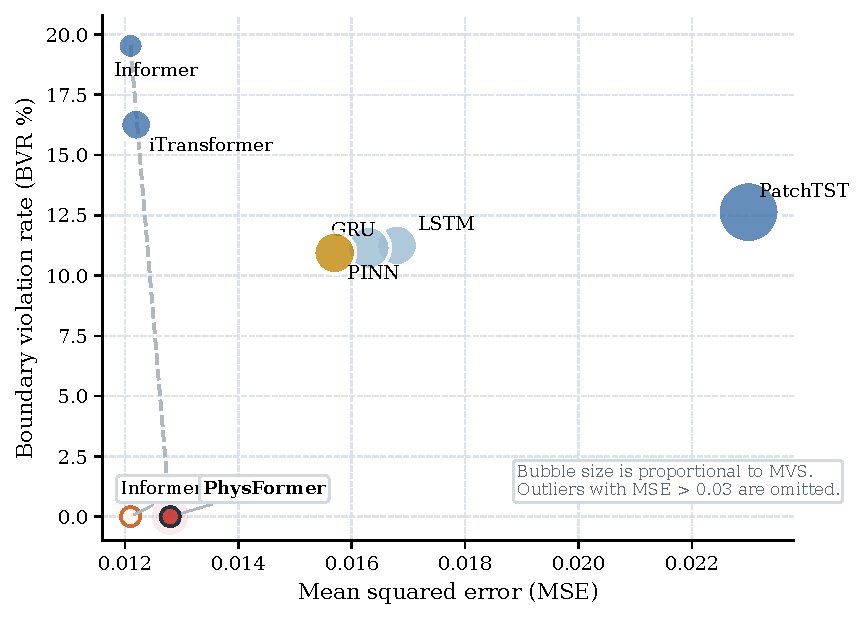
\includegraphics[width=0.98\columnwidth]{EPSR_Fig5_Pareto.pdf}
\caption{PhysFormer combines zero boundary violations with accuracy close to the strongest unconstrained baselines. High-error outliers with MSE $> 0.03$ are omitted.}
\label{fig:pareto}
\end{figure}

\begin{table}[htbp]
\centering
\caption{Forecasting Performance on the Global Test Set}
\label{tab:main_results}
\footnotesize
\setlength{\tabcolsep}{2pt}
\begin{tabular*}{\columnwidth}{@{\extracolsep{\fill}}lccccc@{\extracolsep{\fill}}}
\toprule
Model & MSE & BVR (\%) & MVS (MW) & RVR-S (\%) & NET MAE \\
\midrule
LSTM & 0.0168 & 11.25\% & 0.0093 & 0.01\% & 0.1760 \\
GRU & 0.0163 & 11.15\% & 0.0103 & 0.01\% & 0.1740 \\
PINN & 0.0157 & 10.94\% & 0.0097 & 0.02\% & 0.1702 \\
Informer & \textbf{0.0121} & 19.53\% & 0.0036 & 0.05\% & \textbf{0.1471} \\
Informer-Post & 0.0121 & 0.00\% & 0.0000 & 0.05\% & 0.1471 \\
iTransformer & 0.0122 & 16.26\% & 0.0054 & 0.028\% & 0.1482 \\
Autoformer & 0.1253 & 12.67\% & 0.0737 & \textbf{0.00\%} & 0.4846 \\
DLinear & 0.1015 & 7.03\% & 0.0295 & \textbf{0.00\%} & 0.4279 \\
PatchTST & 0.0230 & 12.63\% & 0.0207 & \textbf{0.00\%} & 0.2052 \\
PhysFormer & 0.0128 & \textbf{0.00\%} & \textbf{0.0000} & 0.198\% & 0.1527 \\
\bottomrule
\end{tabular*}
\end{table}

To make the trade-off concrete, Fig.~\ref{fig:forecast_comparison} focuses on a representative PV forecast window where the shutdown transition is visible within the 96-step horizon. The PV channel is shown here because boundary handling is most transparent in the zero-generation intervals.

\begin{figure}[tbp]
\centering

\includegraphics[width=0.94\columnwidth]{EPSR_Fig6_PVCaseStudy.pdf}
\caption{PhysFormer tracks the PV shutdown transition without crossing the zero boundary. Panel (a) shows the full forecast horizon, and panel (b) zooms into the dusk shutdown window.}
\label{fig:forecast_comparison}
\end{figure}

\FloatBarrier

\subsection{Verification of Physical Compliance and Safety}
\label{subsec:safety}

\subsubsection{Limitations of Heuristic Post-Processing}
\label{subsubsec:compliance}

Table~\ref{tab:main_results} also shows that hard zero-clipping applied to Informer (Informer-Post) reduces BVR to zero without changing the reported MSE. This makes Informer-Post a useful practical baseline rather than a strawman. The difference is structural. Post-processing acts only after prediction, whereas BPAR changes the output parameterization during training and keeps the boundary treatment differentiable.

\subsubsection{Robustness Under Extreme Conditions}
\label{subsubsec:extreme_weather}

To evaluate model stability under stronger distribution shifts, we isolate the top 10\% highest-volatility samples. The corresponding results are listed in Table~\ref{tab:extreme_results}.

Under these conditions, channel-independent architectures such as Autoformer and DLinear degrade more strongly, whereas the competitive tier remains more stable. PhysFormer keeps BVR at $0.00\%$ while remaining close to the best MSE values. We also checked BPAR under seasonal shifts and degenerate variance conditions ($\sigma_x < 10^{-3}$). For the aggregated VPP windows used here ($\text{seq\_len}=672$), such cases do not appear in the test set.

\begin{table}[htbp]
\centering
\caption{Extreme Weather Performance (Top 10\% Volatility)}
\label{tab:extreme_results}
\footnotesize
\setlength{\tabcolsep}{2pt}
\begin{tabular*}{\columnwidth}{@{\extracolsep{\fill}}lccccc@{}}
\toprule
Model & MSE & BVR (\%) & MVS (MW) & RVR-S (\%) & NET MAE \\
\midrule
LSTM & 0.0192 & 13.43\% & 0.0086 & 0.000\% & 0.1941 \\
GRU & 0.0182 & 13.79\% & 0.0097 & 0.000\% & 0.1864 \\
PINN & 0.0177 & 13.29\% & 0.0082 & 0.000\% & 0.1807 \\
Informer & \textbf{0.0146} & 21.38\% & 0.0017 & 0.070\% & \textbf{0.1632} \\
iTransformer & 0.0143 & 19.79\% & 0.0053 & \textbf{0.046\%} & 0.1639 \\
PatchTST & 0.0261 & 12.22\% & 0.0132 & 0.000\% & 0.2240 \\
PhysFormer & 0.0150 & \textbf{0.00\%} & \textbf{0.0000} & 0.294\% & 0.1715 \\
\bottomrule
\end{tabular*}
\end{table}

Fig.~\ref{fig:extreme_weather} shows the same pattern: PhysFormer remains close to the best MSE tier while keeping zero BVR.

\begin{figure}[tbp]
\centering

\includegraphics[width=0.84\columnwidth]{EPSR_Fig7_ExtremeWeather.pdf}
\caption{On the extreme-weather subset, PhysFormer stays near the best MSE tier and is the only model with zero boundary violations.}
\label{fig:extreme_weather}
\end{figure}

\subsection{Model Interpretability and Efficiency}
\label{subsec:mechanism}

\subsubsection{Evaluation of Physical Interpretability}
\label{subsubsec:interpretability}

A key advantage of PhysFormer is that its physical parameters remain readable after training. As shown in Table~\ref{tab:physical_params}, the learned values stay within typical engineering ranges \cite{Li2026,Asinyo2025}. The PV temperature coefficient changes by only $+2.5\%$, and the wind thresholds stay close to their initial priors.

The main quantitative evidence is the alignment between the learned PV gate and irradiance. PGCC yields a global Pearson correlation of $r = 0.8306 \ (p < 0.001)$. On the daytime subset (irradiance $> 0.1$), the correlation remains significant at $r = 0.4058 \ (p < 10^{-57})$.

This behavior should be understood as supervised alignment rather than emergent causality. Under additional sensor-noise tests, the correlation remains at $r = 0.8377$ with 20\% white noise and stays above $0.81$ even when the noise amplitude reaches 50\%.

\subsubsection{Distinction Between Supervised Alignment and Emergent Causality}
It is important to state the limits of this result clearly. The high correlation ($r=0.8306$) does not indicate emergent meteorological causality discovered \textit{ab initio} from raw data. Instead, Gate Response Regularization provides supervised alignment to a known physical prior.

\begin{table}[tbp]
\centering
\caption{Physical Parameter Convergence Tracking}
\label{tab:physical_params}
\scriptsize
\setlength{\tabcolsep}{3pt}
\begin{tabular*}{\columnwidth}{@{\extracolsep{\fill}}lcccc@{}}
\toprule
Parameter & Initial & Converged & Lit. Range & $\Delta$ \\
\midrule
\texttt{pv\_temp\_coef} & 0.0040 & $0.0041/^\circ$C & 0.003--0.005 & $+2.5\%$ \\
\texttt{wind\_cut\_in} & 3.50 m/s & 3.458 m/s & 3--5 m/s & $-1.2\%$ \\
\texttt{wind\_rated} & 12.00 & 11.970 m/s & 10--15 m/s & $-0.2\%$ \\
\texttt{wind\_cut\_out} & 25.00 & 24.968 m/s & 20--25 m/s & $-0.1\%$ \\
\texttt{load\_base} & 2.832 MW & 2.823 MW & $\approx$ mean & $-0.3\%$ \\
\texttt{temp\_comfort} & $20.0^\circ$C & $19.992^\circ$C & 18--22$^\circ$C & $\approx 0$ \\
\bottomrule
\end{tabular*}
\end{table}

\subsubsection{Computational Complexity Analysis}
\label{subsubsec:overhead}

To evaluate computational cost, we compare parameter counts and inference latency under the same hardware setting. As shown in Table~\ref{tab:overhead}, PhysFormer uses $d_\text{model}=512$ but has 11.4M parameters, compared with Informer's 17.9M. The measured latency is about $2.10$ ms/sample on an RTX 3090 GPU.

\begin{table}[!htbp]
\centering
\caption{Model Complexity and Inference Overhead}
\label{tab:overhead}
\scriptsize
\setlength{\tabcolsep}{2pt}
\begin{tabular*}{\columnwidth}{@{\extracolsep{\fill}}lcc@{}}
\toprule
Model & Params (M) & Latency (ms) \\
\midrule
LSTM / GRU & 5.42 / 4.10 & 1.20 / 2.19 \\
PINN / DLinear & 2.74 / 0.13 & $<$0.10 / $<$0.10 \\
Informer / Autoformer & 17.90 / 17.88 & 1.96 / 4.28 \\
PatchTST / iTransformer & 1.62 / 9.85 & 0.10 / 1.81 \\
\textbf{PhysFormer} & \underline{11.4} & \underline{2.10} \\
\bottomrule
\end{tabular*}
\end{table}

\FloatBarrier

\subsection{Ablation Study}
\label{subsec:ablation}

We further evaluate the contribution of each module through an ablation study on the real dataset (Table~\ref{tab:ablation}).

\subsubsection{Component-wise Ablation Analysis}
Table~\ref{tab:ablation} shows four main trends. First, removing the physics stream increases MSE by $4.7\%$, so the theory-based baseline remains useful. Second, removing PGCC leaves MSE unchanged, which is consistent with its role in alignment rather than raw accuracy. Third, removing curriculum training increases MSE by $8.7\%$, which indicates that staged optimization helps. Fourth, removing the future GLU increases MSE by $1.6\%$ while keeping BVR at $0.00\%$, which suggests that future-weather injection mainly improves accuracy around transition periods.

\begin{table}[htbp]
\centering
\caption{Ablation Study on Real Data}
\label{tab:ablation}
\footnotesize
\setlength{\tabcolsep}{3pt}
\begin{tabular*}{\columnwidth}{@{\extracolsep{\fill}}lcccc@{}}
\toprule
Variant & MSE & BVR (\%) & RVM & $r(\text{gate}_{\text{pv}})$ \\
\midrule
Full PhysFormer & 0.0128 & 0.00 & 0.0000 & 0.8306 \\
w/o Physics Stream & 0.0134 & 0.00 & 0.0000 & N/A \\
w/o PGCC & 0.0128 & 0.00 & 0.0000 & N/A \\
w/o Future GLU & 0.0130 & 0.00 & 0.0000 & 0.8024 \\
w/o Curriculum & 0.0139 & 0.00 & 0.0000 & 0.7866 \\
\bottomrule
\end{tabular*}
\end{table}

An additional variant ("w/ PGCC but w/o Gate Response Regularization") keeps a competitive MSE (0.0128) but fails to produce clear gate-weather alignment ($r < 0.12$). This confirms that explicit regularization is the main source of the alignment result.

The evaluation also has clear limits. All experiments are conducted on one aggregated regional dataset with one temporal resolution and one forecasting horizon. The study focuses on component-level forecasting and does not include storage dynamics, state-of-charge constraints, or closed-loop dispatch. The reported interpretability result should therefore be read as supervised alignment to known weather cues, not as causal discovery.
